
\documentclass[runningheads]{llncs}

%========== Packages ==========
\usepackage[utf8]{inputenc}
\usepackage[T1]{fontenc}
\usepackage{microtype}
\usepackage{amssymb}
\usepackage{mathtools}
\usepackage{booktabs}
\usepackage{array}
\usepackage{xspace}
\usepackage[linesnumbered, lined, ruled]{algorithm2e}
\usepackage[inline]{enumitem}
\usepackage[caption=false]{subfig}
\usepackage{tikz}
%\captionsetup{compatibility=false}
\usepackage{float}
%\usepackage{graphicx}
\usepackage{hyperref} \renewcommand\UrlFont{\color{blue}\rmfamily}

%%%%%%%%%% REMOVE BEFORE PUBLISHING %%%%%%%%%%
\usepackage{todonotes}


%========== TikZ setup ==========
\usetikzlibrary{arrows}
\tikzset{auto, >=stealth}


%========== Algorithm2e setup ==========
\SetKwProg{Fn}{Function}{:}{end}
\SetKwProg{Pr}{Procedure}{:}{end}
\SetKwComment{InlineComment}{\textcolor{gray!75}{//} }{}
\SetKwComment{MultilineComment}{\textcolor{gray!75}{/*} }{\textcolor{gray!75}{ */}}
\SetKwFunction{RelevantPredicates}{Relevant-Predicates}
\SetKwFunction{SorcarPassive}{Sorcar-Passive}
\SetKwFunction{SorcarIterative}{Sorcar-Iterative}
\SetKwFunction{RelevantPredicatesMax}{Relevant-Predicates-Max}
\SetKwFunction{RelevantPredicatesFirst}{Relevant-Predicates-First}
\SetKwFunction{RelevantPredicatesMin}{Relevant-Predicates-Min}
\SetKwFunction{RelevantPredicatesGreedy}{Relevant-Predicates-Greedy}


%========== Macros ==========
\newcommand{\houdini}{\textsc{Houdini}\xspace}
\newcommand{\sorcar}{\textsc{Sorcar}\xspace}
\newcommand{\boogie}{\textsc{Boogie}\xspace}


%========== Meta data ==========

%---------- Title ----------
\title{\textsc{Sorcar}: Property-Driven Algorithms for Learning Small Conjunctive Invariants%\thanks{Supported by organization x.}
}
\titlerunning{\textsc{Sorcar}: Property-Driven Algorithms for Learning Small Conjuncts} %If the paper title is too long

%---------- Authors ----------
\author
{
    Anonymous Authors
}
\authorrunning{Anonymous authors}

%---------- Institutes ----------
%\institute
%{
%    Anonymous Institution \and
%    Anonymous Institution
%}

\institute
{
    ~
}

%========== Document begins here ==========
\begin{document}

%---------- Title ----------
\maketitle

%---------- Abstract ----------
\begin{abstract}
We present a new learning algorithm \sorcar to synthesize conjunctive invariants for proving a program satisfies its assertions. The new algorithm is property-driven and is biased towards learning smaller conjunctive invariants over a fixed finite set of $n$ predicates, guarantees convergence in $2n$ rounds, and takes only polynomial time in each round. We implement and evaluate the algorithm and show that its performance is favorable to the existing \houdini algorithm for a class of benchmarks that prove data race freedom of GPU programs and another class that synthesizes invariants for proving separation logic properties for heap manipulating programs.
\keywords{Invariant Synthesis \and Machine Learning \and Horn-ICE Learning \and Conjunctive Formulas.}
\end{abstract}


%========== Content ==========

%\textcolor{blue}{Page limit is 16 pages, not counting references and appendices. Double-blind.}

%---------- Introduction ----------
% !Tex root=main.tex

\section{Introduction}
\label{sec:intro}

The deductive verification approach for proving imperative programs correct is one of the most well-established and effective methods, and automating program verification using this method has been studied extensively. This approach can be seen as consisting of two parts:
\begin{enumerate*}[label={(\alph*)}]
    \item writing inductive invariants in terms of loop invariants, class invariants, and method contracts, and
    \item proving that these annotations are indeed correct using theorem proving.
\end{enumerate*} 
Automation of the latter has seem tremendous progress in the last two decades through the identification of decidable logical theories, theory combinations, heuristics for automatically reasoning with quantified theories, and their realization using efficient SMT solvers~\cite{DBLP:conf/cav/BarrettCDHJKRT11,DBLP:conf/tacas/MouraB08}.
There has also been significant progress on automating the former problem of discovering inductive invariants~\cite{DBLP:conf/pldi/BallMMR01,DBLP:conf/vmcai/Bradley11,DBLP:conf/tacas/ChampionC0S18,DBLP:conf/cav/ColonSS03,DBLP:conf/popl/CousotC77,DBLP:conf/oopsla/DilligDLM13,DBLP:conf/icse/ErnstCGN00,DBLP:journals/pacmpl/EzudheenND0M18,DBLP:conf/fm/FlanaganL01,DBLP:conf/fmcad/FedyukovichKB17,DBLP:conf/cav/0001LMN13,DBLP:conf/cav/0001LMN14,DBLP:conf/pldi/GulwaniSV08,DBLP:conf/cav/GuptaR09,DBLP:journals/corr/KrishnaPW15,DBLP:conf/cav/McMillan03,DBLP:conf/cav/0001A14,DBLP:conf/esop/0001GHALN13,DBLP:conf/sas/0001GHAN13,DBLP:conf/cav/SharmaNA12,DBLP:conf/pldi/ZhuMJ18}, with varying degrees of success. 

In this paper, we are interested in a class of \emph{black-box} or \emph{learning-based} techniques for invariant generation~\cite{DBLP:conf/tacas/ChampionC0S18,DBLP:journals/pacmpl/EzudheenND0M18,DBLP:conf/cav/0001LMN14,DBLP:conf/pldi/ZhuMJ18}. In this context, the invariant synthesis engine is split into two components, a learner and a teacher, who work in rounds. In each round, the teacher examines the invariant produced by the learner and produces counterexamples that consist of concrete program configurations that show why the proposed formulas are not inductive invariants. The learner then uses these concrete program configurations to synthesize new proposals for the invariant, \emph{without} looking at the program. The teacher, on the other hand, does look at the program and essentially produces counterexamples using failed verification attempts of the program.

The choice to separate the learner and teacher---and not give the learner access to the program---may seem strange at first.
However, a rationale for this choice has emerged over the years, and the above choice is in fact the \textit{de~facto} approach for synthesis in various other domains, including program synthesis, where it is usually called counter-example guided inductive synthesis~\cite{DBLP:series/natosec/AlurBDF0JKMMRSSSSTU15,cegis,DBLP:conf/asplos/Solar-LezamaTBSS06}.

%Intuitively, synthesis problems, including invariant synthesis, can be seen as solving $\exists^\ast \forall^\ast$ problems (does there exists an invariant/expression $E$ such that for every valuation of variables, a specification $\varphi(E)$ holds).
%Such problems are hard to solve, and the split into two components reduces it to an iterative scenario where each component is solving a problem that has no quantifier alternation.
%In the invariant synthesis setting, for instance, the learner is solving the problem of whether there exists an expression that satisfies all the concrete counterexamples, while the teacher is solving the problem of whether there exists a counterexample that shows the proposed formula is not an inductive invariant, both being $\exists^\ast$ problems.

\paragraph{\bfseries Horn-ICE Learning}
In a paper at CAV 2014, Garg et al.~\cite{DBLP:conf/cav/0001LMN14} studied the above learning model and identified the precise form of counterexamples needed for synthesizing invariants---contrary to usual classification learning where one is given positive and negative examples only, the authors argued that implication counterexamples (ICE) are needed, and coined the term \emph{ICE learning} for such a learning model.
More recently, it has been recognized that program verification problems can be cast as solving \emph{Horn implication constraints}.
Consequently, the implication counterexamples returned by the teacher are naturally Horn implications (\emph{Horn-ICE}), involving concrete program configurations, and new learning algorithms for learning from such Horn counterexamples have recently been studied~\cite{DBLP:conf/tacas/ChampionC0S18,DBLP:journals/pacmpl/EzudheenND0M18}.
 
\paragraph{\bfseries Learning Conjunctions}
While one can potentially learn/synthesize invariants in over complex logics, one technique that has been particularly effective and scalable is to fix a finite set of predicates $\mathcal P$ over the program configurations and only learn invariants that can be expressed as a conjunction of a subset of these predicates.
For programs over particular domains and particular classes of specifications, where the typical class of predicates needed is known, these techniques often work very well. 

We are motivated by two such domains. The first is the class of programs handled by GPUVerify~\cite{DBLP:conf/oopsla/BettsCDQT12,DBLP:conf/oopsla/ChongDKKQ13}, which considers GPU programs with parallelism, reduces the problem to a sequential verification problem (by simulating two threads at each parallel fork), and proceeds to find inductive invariants over a fixed class $\mathcal P$ to prove the resulting sequential program correct.
The second class is the class of programs considered by Neider et al.~\cite{DBLP:conf/tacas/Neider0MS018}, where the authors synthesize invariants that express properties of heaps in order to prove programs that dynamically update heaps correct against separation logic specifications.
The verification engine in the former is an SMT solver that returns concrete Horn-ICE counterexamples and in the latter is an incomplete verification engines that returns abstract counterexamples that can be interpreted to be Horn-ICE counterexamples. 
In both domains, the set $\mathcal P$ consists of hundreds of predicates, which makes invariant synthesis challenging.

\paragraph{\bfseries \houdini and \sorcar}
The classical algorithm for learning conjunctive invariants over a finite class of predicates is the \houdini algorithm~\cite{DBLP:conf/fm/FlanaganL01}, which mimics the \emph{elimination algorithm} for learning conjuncts in classical machine learning~\cite{Kearns:1994:ICL:200548}.
\houdini starts with a conjectured invariant that contains \emph{all} predicates and, in each round, uses counterexamples to remove predicates.
On the positive side, the algorithm is guaranteed to construct the \emph{minimal} inductive invariant expressible as a conjunction over $\mathcal P$ and takes at most $n=|\mathcal P|$ rounds to converge to such an inductive invariant, if one exists. 

However, the \houdini algorithm has disadvantages as well.
First, it is not property driven (i.e., it does not consider the assertions that occur in the program).
Secondly, as a consequence, it synthesizes invariants that have the \emph{largest} number of conjuncts (i.e., the semantically smallest sets of program configurations expressible as a conjunctive formula).

\emph{In this paper, we develop a new class of algorithms, which we call \sorcar\footnote{Houdini and Sorcar were both magicians!}, that is \emph{property-driven} and aims to learn \emph{small conjunctions}.} 

%Unfortunately, learning small conjunctions efficiently in an online setting interacting with a teacher is hard.
%When only positive and negative samples are present, there is a beautiful algorithm called the Winnow algorithms that can learn conjunctive formula in $O(r \log n)$ rounds where $r$ is the number of conjuncts in the smallest formula consistent with the eventually learned formula.
%However, an extension of this algorithm to the ICE/Horn-ICE setting seems very difficult (more precisely, has not yielded to the efforts of the authors of this paper in consultation with machine language theory people for more than a year). 

\begin{table}[t]
	\caption{Comparison of \houdini~\cite{DBLP:conf/fm/FlanaganL01} and \sorcar} \label{tab:learners_comparison}
	\centering
	%\footnotesize
	\begin{tabular}{l@{\hskip 1em}c@{\hskip 1em}c@{\hskip 1em}c@{\hskip 1em}m{35mm}}
		\toprule
		\multicolumn{1}{c}{\textbf{Learning}} & \textbf{Property} & \textbf{Complexity} & \textbf{Maximum} & \multicolumn{1}{c}{\textbf{Final conjunct}} \\
		\multicolumn{1}{c}{\textbf{algorithm}} & \textbf{driven?} & \textbf{per round} & \textbf{\# rounds} & \\
		\midrule
		\houdini & No & Polynomial & $|\mathcal P|$ & Largest set \\\addlinespace
		\midrule
		\sorcar & Yes & Polynomial & $2 \cdot |\mathcal P|$ & Bias towards smaller sets involving only relevant predicates \\
		\bottomrule
	\end{tabular}
\end{table}

The \sorcar algorithm presented in this paper has the following features (see Table~\ref{tab:learners_comparison}).
First, it guarantees that the number of rounds of interaction with the teacher is still linear ($2n$ rounds compared to Houdini's promise of $n$ rounds).
Second, it is property-driven---in other words, the algorithm tries to find the smallest conjunctive inductive invariant that satisfies the assertions in the program. There is no guarantee though on how small the invariant will be (in experiments, we show how it achieves small invariants).
Third, it promises to do only polynomial amount of work in each round (i.e., polynomial in $n$ and in the number of current counterexamples), similar to \houdini. 

We believe that the \sorcar algorithm is a new learning algorithm with interesting properties and guarantees for learning conjunctive invariants. 

\paragraph{\bfseries Experimental evaluation}
The \sorcar algorithm is certainly well suited for applications where property-driven invariants are expected to be small and one wishes to learn small invariants.
Learning small invariants can be particularly useful in applications where these algorithms are used to \emph{mine specifications} that a user may read.
For example, if we use \sorcar to mine provable contracts for methods, then contracts would be easier to read if they are smaller (i.e., contain less predicates).
However, even when invariants are not required to be small, \sorcar is a new algorithm that, being property-driven, can be more effective. 

We have implemented \sorcar as a Horn-ICE learning algorithm interacting with the \boogie program verifier and have applied it to verify both GPU programs for data races~\cite{DBLP:conf/oopsla/BettsCDQT12,DBLP:conf/oopsla/ChongDKKQ13} and heap manipulating programs against separation logic specifications~\cite{DBLP:conf/tacas/Neider0MS018}, and compare them with the current state-of-the-art for these tools that use the \houdini algorithm.
Using large classes of programs, we show that
\begin{enumerate*}[label={(\alph*)}]
    \item \sorcar produces much smaller invariants %\textcolor{orange}{(...)},
    \item works faster overall in verifying these programs, and
    \item verifies more programs than \houdini does.
\end{enumerate*}
\sorcar does not, of course, perform faster on all programs or always produce small invariants---however, it certainly emerges as a new competitive algorithm that shows significant advantages in all fronts for many programs.

% !Tex root=main.tex

\subsection*{Related Work}
Invariant synthesis lies at the heart of automated program verification.
Over the years, various techniques have been proposed, including abstract interpretation~\cite{DBLP:conf/popl/CousotC77}, interpolation~\cite{DBLP:conf/cav/McMillan03}, IC3~\cite{DBLP:conf/vmcai/Bradley11}, predicate abstraction~\cite{DBLP:conf/pldi/BallMMR01}, abductive inference~\cite{DBLP:conf/oopsla/DilligDLM13}, as well as synthesis algorithms that rely on constraint solving~\cite{DBLP:conf/cav/ColonSS03,DBLP:conf/fmcad/FedyukovichKB17,DBLP:conf/pldi/GulwaniSV08,DBLP:conf/cav/GuptaR09}.
Complementing these techniques are data-driven approaches that are based on machine learning.
Examples include \textsc{Daikon}~\cite{DBLP:conf/icse/ErnstCGN00} and \houdini~\cite{DBLP:conf/fm/FlanaganL01}, the ICE learning framework~\cite{DBLP:conf/cav/0001LMN14} and its successor Horn-ICE learning~\cite{DBLP:conf/tacas/ChampionC0S18,DBLP:journals/pacmpl/EzudheenND0M18}, as well as numerous other techniques that employ machine learning to synthesize inductive invariants~\cite{DBLP:conf/cav/0001LMN13,DBLP:journals/corr/KrishnaPW15,DBLP:conf/cav/0001A14,DBLP:conf/esop/0001GHALN13,DBLP:conf/sas/0001GHAN13,DBLP:conf/cav/SharmaNA12,DBLP:conf/pldi/ZhuMJ18}.

%\textcolor{red}{Why conjunctive invariants?}
%Focusing on conjunctive invariants has proven to be an effective strategy in practice.
% Two exmples hwere ristricting the class of 
% Some require richer conept classes. Recently decision trees (move to end of section?).

Learning of conjunctive formulas has a long history.
An early example is the so-called elimination algorithm~\cite{Kearns:1994:ICL:200548}, which operates in the Probably Approximately Correct Learning model (PAC).
\textsc{Daikon}~\cite{DBLP:conf/icse/ErnstCGN00} was the first technique to apply the elimination algorithm in a software setting, learning likely invariants from dynamic traces.
Later, the popular \houdini~\cite{DBLP:conf/fm/FlanaganL01} algorithm built on top of the elimination algorithm to learn inductive invariants in a fully automated manner.
In fact, as Garg et al.~\cite{Garg:2016} and later Ezudheen et al.~\cite{DBLP:journals/pacmpl/EzudheenND0M18} argued, \houdini can be seen as a learning algorithm for conjunctive formulas in both the ICE and the Horn-ICE learning framework.
However, a drawback of \houdini is that it is not property-driven and does not consider the annotations in the program; instead, \houdini always computes the largest inductive invariant in terms of the number of conjuncts. 
Our novel \sorcar algorithm addresses this shortcoming of \houdini and is designed to learn smaller conjunctive invariants by explicitly taking the assertions in a program into account.

%---------- Background ----------
% !Tex root=main.tex

\section{Background}
\label{sec:background}

In this section, we provide the background on learning-based invariant synthesis.
In particular, we briefly recapitulate the Horn-ICE learning framework (in Section~\ref{sec:horn-ICE}) and discuss the \houdini algorithm (in Section~\ref{sec:houdini}).

To make the Horn-ICE framework mathematically precise, let $P$ be the program (with assertions) under consideration and $\mathcal C$ the set of all program configurations of $P$.
Furthermore, let us fix a finite set $\mathcal P$ of \emph{predicates}
$p \colon \mathcal C \to \mathbb B$ over the program configurations, where $\mathbb B = \{ 0, 1 \}$ is the set of Boolean values (with $1$ interpreted as \textit{true} and $0$ as \textit{false}).
These predicates capture interesting properties of the program and serve as the basic building blocks for constructing invariants.
We assume that the values of these predicates can either be obtained directly from the program configurations or that the program is instrumented with ghost variables that track the values of the predicates at important places in the program (e.g., at the loop header and immediately after the loop).
As notational convention, we write $c \models p$ if $p(c) = 1$ and $c \not\models p$ if $p(c) = 0$.
Moreover, we lift this notation to formulas $\varphi$ over $\mathcal P$ (i.e., arbitrary Boolean combinations of predicates from $\mathcal P$) and use $c \models \varphi$ ($c \not\models \varphi$) to denote that $c$ satisfies $\varphi$ ($c$ does not satisfy $\varphi$), that is defined as usual. 
%We assume that one can evaluate predicates on a program configuration in constant time.

To simplify the presentation in the remainder of this paper, we use conjunctions $p_1 \land \cdots \land p_n$ of predicates over $\mathcal P$ and the corresponding sets $\{ p_1, \ldots, p_n \} \subseteq \mathcal P$ interchangeably.
In particular, for a (sub-)set $X = \{ p_1, \ldots, p_n \} \subseteq \mathcal P$ of predicates and a program configuration $c \in \mathcal C$, we write $c \models X$ if and only if $c \models p_1 \land \cdots \land p_n$.


%---------- The Horn-ICE Learning Framework ----------
\subsection{The Horn-ICE Learning Framework}
\label{sec:horn-ICE}

The Horn-ICE learning framework~\cite{DBLP:conf/tacas/ChampionC0S18,DBLP:journals/pacmpl/EzudheenND0M18} is a general framework for learning inductive invariants in a black-box setting.
We here assume without loss of generality that the task is to synthesize a single invariant.
In the case of learning multiple invariants, say at different program locations, one can easily expand the given predicates to predicates of the form $(\mathit{pc} = l) \rightarrow p$ where $\mathit{pc}$ refers to the program counter, $l$ is the location of an invariant in the program, and $p \in \mathcal P$.
Learning a conjunctive invariant over this extended set of predicates then corresponds to learning multiple conjunctive invariants at the various locations. % in the program.

As sketched in Figure~\ref{fig:horn-ice-learning}, this framework consists of two distinct entities---the \emph{learner} and the \emph{teacher}---and proceeds in rounds.
%In each round, the learner proposes a candidate invariant $\varphi$ for the program, and the teacher, with access to a verification engine, checks whether the proposed invariant proves the program correct. 
%If this is the case, the learning process stops, and this invariant is returned.
%If, on the other hand, the invariant is not adequate to prove the program correct, the teacher replies with concrete program configurations (so called \emph{counterexamples}), which the learner then uses in the next round to refine its conjecture.
%Note that the key feature of this framework is that the learner is completely agnostic of the program and the specification---it is simply constrained to learn some predicate that is consistent with the counterexamples given by the teacher.
%
In each round, the teacher receives a candidate invariant $\varphi$ from the learner and checks whether $\varphi$ proves the program correct.
Should $\varphi$ not be adequate to prove the program correct, the learner replies with a counterexample, which serves as a means to correct inadequate invariants and guide the learner towards a correct one.
More precisely, a counterexample takes one of three forms:\footnote{By abuse of notation, we write $c \models \alpha$ ($c \not\models \alpha$) to denote that $c$ satisfies (violates) the formula $\alpha$ even if $\alpha$ contains predicates that do not belong to $\mathcal P$.}
\begin{itemize}
    \item If the pre-condition $\alpha$ of the program does not imply $\varphi$, then the teacher returns a \emph{positive counterexample} $c \in \mathcal C$ such that $c \models \alpha$ but $c \not \models \varphi$.
    %
    \item If $\varphi$ does not imply the post-condition $\beta$ of the program, then the teacher returns a \emph{negative counterexample} $c \in \mathcal C$ such that $c \models \varphi$ but $c \not \models \beta$.
    %
     \item If $\varphi$ is not inductive, then the teacher returns a \emph{Horn counterexample} $(\{ c_1, \ldots, c_n \}, c) \in 2^\mathcal C \times \mathcal C$ such that $c_i \models \varphi$ for each $i \in \{ 1, \ldots, n \}$ but $c \not\models \varphi$. (We encourage the reader to think of Horn counterexamples as constraints of the form $(c_1 \land \cdots \land c_n) \rightarrow c$.)
\end{itemize}

\begin{figure}[t]
    \centering
    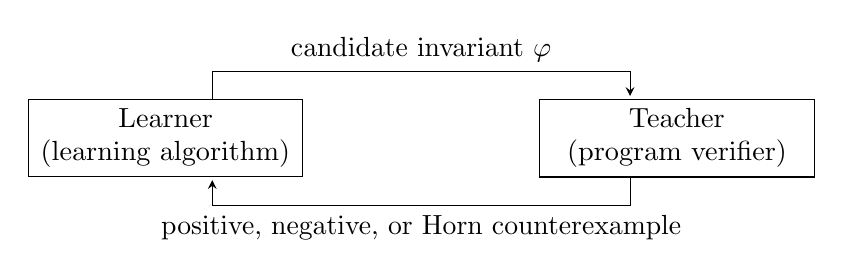
\begin{tikzpicture}
        \node[draw, text width=32.5mm, align=center, anchor=east] (learner) at (0, 0) {Learner \\ (learning algorithm)};
        \node[draw, text width=32.5mm, align=center, anchor=west] (teacher) at (3, 0) {Teacher \\ (program verifier)};
        
        \begin{scope}[->, shorten >= 1pt]
            \draw (learner.40) -- ++(0, .35) -| node[near start] {candidate invariant $\varphi$} (teacher.140);
            \draw (teacher.220) -- ++(0, -.35) -| node[near start] {positive, negative, or Horn counterexample} (learner.320);
        \end{scope}
    \end{tikzpicture}
    \caption{The Horn-ICE learning framework~\cite{DBLP:conf/tacas/ChampionC0S18,DBLP:journals/pacmpl/EzudheenND0M18}}
    \label{fig:horn-ice-learning}
\end{figure}

A teacher who returns counterexamples as described above always enables the learner to make \emph{progress} in the sense that every counterexample it returns is inconsistent with the current conjecture.
Moreover, the Horn-ICE framework requires the teacher to be \emph{honest}, meaning that each counterexample needs to be consistent with \emph{all} inductive invariants that prove the program correct (i.e., the teacher does not rule out possible solutions).
Finally, note that such a teacher can indeed be built since program verification can be stated using \emph{constrained Horn clauses}~\cite{DBLP:conf/pldi/GrebenshchikovLPR12}.
When the candidate invariant does not make such clauses true, some Horn clause must fail, and the teacher can find a Horn counterexample using a logic solver (positive counterexamples arise when the left-hand-side of the Horn counterexample is empty, while negative counterexamples arise when the left-hand-side has one element and the-right-hand side is \emph{false}).


The objective of the learner, on the other hand, is to construct a formula $\varphi$ over $\mathcal P$ from the counterexamples received thus far.
For the sake of simplicity, we assume that the learner collects all counterexamples in a data structure $\mathcal S = (S_+, S_-, S_H)$, called \emph{Horn-ICE sample}, where
\begin{enumerate*}[label={(\alph*)}]
    \item $S_+ \subseteq \mathcal C$ is a finite set of positive counterexamples,
    \item $S_- \subseteq \mathcal C$ is a finite set of negative counterexamples, and
    \item $S_H \subseteq 2^\mathcal C \times \mathcal C$ is a finite set of Horn counterexamples.
\end{enumerate*}
To measure the complexity of a sample, we define its \emph{size}, denoted by $|\mathcal S|$, to be $|S_+| + |S_-| + \sum_{(L, c) \in S_H} (|L| + 1)$.

Given a Horn-ICE sample $\mathcal S = (S_+, S_-, S_H)$, the learner's task is then to construct a formula $\varphi$ over $\mathcal P$ that is \emph{consistent} with $\mathcal S$ in that
\begin{enumerate*}[label={(\alph*)}]
    \item $c \models \varphi$ for each $c \in S_+$,
    \item $c\not \models \varphi$ for each $c \in S_-$, and
    \item for each $(\{ c_1, \ldots, c_n \}, c) \in S_H$, if $c_i \models \varphi$ for all $i \in \{ 1, \ldots, n \}$, then $c \models \varphi$.
\end{enumerate*}
This task is called \emph{passive Horn-ICE learning}, while the overall learning setup can be though of as \emph{iterative (or online) Horn-ICE learning}.
In the special case that the learner produces conjunctive formulas, we say that a set $X \subseteq \mathcal P$ is consistent with $\mathcal S$ if and only if the corresponding conjunction $\bigwedge_{p \in X} p$ is consistent with $\mathcal S$


In general, the Horn-ICE learning framework permits arbitrary formulas over the predicates as candidate invariants.
In this paper, however, we exclusively focus on conjunctive formulas (i.e., conjunctions of predicates from $\mathcal P$). % \textcolor{orange}{and assume that the set of predicates is finite}.
In fact, conjunctive invariants form an important subclass in practice as they are sufficient to prove many programs correct~\cite{DBLP:conf/fm/FlanaganL01,DBLP:conf/tacas/Neider0MS018} (also see our experimental evaluation in Section~\ref{sec:experiments}).
Moreover, once can design efficient learning algorithms for conjunctive Boolean formulas, as we show next.


%---------- Houdini ----------
\subsection{\houdini as a Horn-ICE Learning Algorithm}
\label{sec:houdini}

\houdini~\cite{DBLP:conf/fm/FlanaganL01} is typically seen as a particular way to synthesize invariants, but is best understood as a passive Horn-ICE learner for conjuncts, as we describe below.
In fact, \houdini is similar to the classical PAC learning algorithm for conjunctions~\cite{Kearns:1994:ICL:200548}, but extended to work with Horn counterexamples as well.
%In every round, the \houdini algorithm learns the \emph{largest} set of conjuncts that satisfies the current positive and implication samples (thus, it can never misclassify a negative sample if a consistent conjunction exists), and hence learns, in the iterative setting, the invariant that can be expressed using the largest set of conjuncts.

We now describe the \houdini algorithm, as it will be used in the design of the \sorcar algorithm that we develop.
Given a Horn-ICE sample $\mathcal S = (S_+, S_-, S_H)$, \houdini computes the largest conjunctive formula $X \subseteq \mathcal P$ in terms of the number of predicates in $X$ (i.e., the semantically smallest set of program configurations expressible by a conjunctive formula) that is consistent with $\mathcal S$.
Starting with the set $X = \mathcal P$ of all predicates, the \houdini algorithm proceeds as follows:
\begin{enumerate}
    \item \label{item:houdini-1} \houdini removes all predicates $p \in X$ from $X$ that violate a positive counterexample (i.e., there exists a positive counterexample $c \in S_+$ such that $c \not\models p$).
    The result is the unique largest set $X$ of predicates---alternatively the largest conjunctive formula---that is consistent with $S_+$ (i.e., $c \models X$ for all $c \in S_+$).
    %
    \item \label{item:houdini-2} \houdini checks whether all Horn counterexamples are satisfied.
    If a Horn counterexample $(\{ c_1, \ldots, c_n \}, c) \in S_H$ is not satisfied, it means that each program configuration $c_i$ of the left-hand-side satisfies $X$, but the configuration $c$ on the right-hand-side does not.
    However, $X$ corresponds to the semantically smallest set of program configurations expressible by a conjunctive formula that is consistent with $S_+$.
    Moreover, all program configurations $c_i$ on the left-hand-side of the Horn counterexample also satisfy $X$.
    Thus, the right-hand-side $c$ necessarily has to satisfy $X$ as well (otherwise $X$ would not satisfy the Horn counterexample).
    To account for this, \houdini adds $c$ as a new positive counterexample to $S_+$.
    %
    \item \label{item:houdini-3} \houdini repeats Steps~\ref{item:houdini-1} and \ref{item:houdini-2} until a fixed point is reached. Once this happens, $X$ is the unique largest set of predicates that is consistent with $S_+$ and $S_H$.
\end{enumerate}
Finally, \houdini checks whether each negative counterexample violates $X$ (i.e., $c \not\models X$ for each $c \in S_-$).
If this is the case, $X$ is the largest set of predicates that is consistent with $\mathcal S$; otherwise, no consistent conjunctive formula exists.

%Given a Horn-ICE sample $\mathcal S = (S_+, S_-, S_H)$, \houdini computes the largest conjunctive formula $\varphi$ in terms of the number of predicates occurring in $\varphi$ (i.e., the semantically strongest conjunctive formula) that is consistent with $\mathcal S$ in the following way.
%First, it computes the largest conjunction $\varphi$ that is consistent with the positive examples (i.e., $c \models \varphi$ for all $c \in S_+$); note that this conjunction is unique.
%Next, \houdini checks whether the implications are satisfied.
%If this is not the case, then we know for each non-satisfied implication $(\vec{v}_1, \vec{v}_2) \in S_\Rightarrow$ that $\vec{v}_2$ has to be classified positively because $\vec{v}_1$ belongs to every set that includes $S_+$.
%Hence, \houdini adds all such $\vec{v}_2$ to $S_+$, resulting in a new set $S'_+$.
%Subsequently, it constructs the largest conjunction $\varphi'$ that is consistent with the positive examples in $S'_+$ (i.e., $\vec{v} \models \varphi'$ for all $\vec{v} \in S'_+$).
%\houdini repeats this procedure until it arrives at the largest conjunctive formula $\varphi^\ast$ that is consistent with $S_+$ and $S_\Rightarrow$ (again, note that this set is unique).
%Finally, \houdini checks whether each negative example violates $\varphi^\ast$  (i.e., $\vec{v} \not\models \varphi^\ast$ for all $\vec{v} \in S_-$).
%If this is the case, $\varphi^\ast$ is the largest conjunctive formula over $\mathcal B$ that is consistent with $\mathcal S$; otherwise, no consistent conjunctive formula exists.

It is not hard to verify that the time \houdini spends in each round is \emph{polynomial} in the number of predicates and the size of the Horn-ICE sample (provided predicates can be evaluated in constant time).
Furthermore, \houdini is guaranteed to converge in at most $|\mathcal P|$ rounds when used in an iterative setting, or it reports that no conjunctive invariant over $\mathcal P$ exists.

The property that \houdini converges in at most $|\mathcal P|$ rounds is of great importance in practice.
We can, for instance, in every round learn the \emph{smallest} set of conjuncts satisfying the sample, say using a SAT solver.
Doing so would not significantly increase the time taken for learning in each round (thanks to highly-optimized SAT solvers), but the worst-case number of iterations to converge to an invariant becomes exponential.
An exponential number of rounds, however, makes learning invariants often intractable in practice (we implemented such a SAT-based learner, but it performed poorly on our set of benchmarks).
Hence, it is important to keep the number of iterations small when learning invariants.
%, and as we shall show in experiments later, is very advantageous in practice when learning from a large set of predicates.  
Note that the \houdini algorithm does not use \emph{negative examples} to learn formulas, and hence is \emph{not property-driven} (negative examples come from configurations that lead to violating assertions).
The \sorcar algorithm, which we describe in the next section 
%uses negative examples, is property driven, and still has the guarantee of linear number of rounds.
has this feature, but at the same time has a bias to producing small conjunctive invariants.


%---------- Sorcar ----------
% !TeX root = main.tex

%---------- Sorcar ----------
\section{The \sorcar Horn-ICE Learning Algorithm}
\label{sec:sorcar}

One major disadvantage of \houdini is that it learns in each round the largest set of conjuncts, \emph{independent} of negative counterexamples, and hence independent of the assertions and specifications in a program--- it learns the semantically smallest inductive invariant expressible as a set of conjuncts over $\mathcal P$.
This motivates the development of our novel \sorcar Horn-ICE learning algorithm for conjuncts, which is property-driven (i.e., it also considers the assertions in the program) and has a bias towards learning small invariants.
%However, the \sorcar algorithm is more complex and subtle than \houdini, and its correctness proof is more involved.

The salient feature of \sorcar is that it always learns invariants involving what we call \emph{relevant} predicates, which are predicates that have shown some evidence to affect the assertions in the program.
More precisely, we say that a predicate is \emph{relevant} if it evaluates to \textit{false} on some negative counterexample or on a program configuration appearing on the left-hand-side of a Horn counterexample.
This indicates that \emph{not} assuming this predicate leads to an assertion violation or the invariant not being inductive, and is hence deemed important as a candidate predicate in the synthesized invariant.
However, naively choosing relevant predicates does in general lead to an exponential number of rounds.
Thus, \sorcar is designed to select relevant predicates carefully and requires at most $2 |\mathcal P|$ rounds to converge to an invariant (which is twice the number that \houdini guarantees).
Moreover, the set of predicates learned by \sorcar is always a subset of those learned by \houdini.

Algorithm~\ref{alg:sorcar} presents the \sorcar Horn-ICE learner in pseudo code.
In contrast to \houdini, it is not a purely passive learning algorithm but is divided into a passive part (\SorcarPassive) and an iterative part (\SorcarIterative), the latter being invoked in every round of the Horn-ICE framework.
More precisely, \SorcarIterative maintains a state in form of a set $R \subseteq \mathcal P$ in the course of the iterative learning, which is empty in the beginning and used to accumulate \emph{relevant predicates} (Line~\ref{sorcar:line:initialize-R}).
The exact choice of relevant predicates, however, is delegated to an external function \RelevantPredicates.
We treat this function as a parameter for the \sorcar algorithm and discuss four possible implementations at the end of this section.
%The conjunction \sorcar returns is always a subset of these relevant predicates, which is guaranteed to be consistent with the Horn-ICE sample.
%In the beginning of the iterative learning, when the Horn-ICE sample $\mathcal S$ is empty, $R$ is also empty.
Let us now present \sorcar in detail.

\begin{algorithm}[t]

    % Choose relevant predicates
    \label{sorcar:line:relevant-predicates-start}
    %\MultilineComment{\color{gray!75}Computes a set of relevant predicates for a set $N$ of negative counterexamples and a set $H$ of Horn counterexamples}
    \Fn{\RelevantPredicates{$N$, $H$, $X$, $R$}}
    {
        \Return{a set of $R' \subseteq \mathcal P$ of relevant predicates such that $R'\setminus R \neq \emptyset$}\;
    }
    \label{sorcar:line:relevant-predicates-end}

    \BlankLine
    \BlankLine

    % Sorcar passive
    \Pr{\SorcarPassive{$\mathcal S = (S_+, S_-, S_H)$, $R$}}
    {
        $X \gets \{ p_1, \ldots, p_n \}$ such that $\bigwedge_{i=1}^n p_i$ is the largest conjunctive formula over $\mathcal P$ that is consistent with $\mathcal S$ (\KwSty{abort} if no such formula exists)\;
        \label{sorcar:line:largest-conjunction}

        \BlankLine

        \While{$X \cap R$ is not consistent with $\mathcal S$ \label{sorcar:line:loop-head}}
        {

            $N \gets \emptyset$%
            \InlineComment*[r]{\color{gray}Stores inconsistent negative counterexamples}
            \label{sorcar:line:inconsistent-collextion-start}
            $H \gets \emptyset$%
            \InlineComment*[r]{\color{gray}Stores inconsistent Horn counterexamples}
        
            \BlankLine
    

            \ForEach{negative counterexample $c \in S_-$ not consistent with $X \cap R$}
            {
  	        	$N \gets N \cup \{ c \}$\;
            }
            \ForEach{Horn counterexample $(L, c) \in S_H$ not consistent with $X \cap R$}
            {
  	        	$H \gets H \cup \{ (L, c) \}$\;
            }
            \label{sorcar:line:inconsistent-collextion-end}
        
            \BlankLine
        
            $R \gets R \cup {}$\RelevantPredicates{$N$, $H$, $X$, $R$}\;
            \label{sorcar:line:extend-R}

        }
        \label{sorcar:line:loop-end}

        \BlankLine
        
        \Return{$(X \cap R, R)$}\;
    }

    \BlankLine
    \BlankLine

    % Sorcar iterative
    \KwSty{static} $R \gets \emptyset$%
    \InlineComment*[r]{\color{gray!75}Stores relevant predicates across rounds}
    \label{sorcar:line:initialize-R}
    
    \BlankLine
    
    \Pr{\SorcarIterative{$\mathcal S$}}
    {
        
        $(Y, R) \gets {}$\SorcarPassive{$\mathcal S, R$}\;
        \Return{$Y$}\;
        
    }
    
    \caption{The \sorcar Horn-ICE learning algorithm}
    \label{alg:sorcar}
    
\end{algorithm}


%---------- Sorcar Passive ----------
\paragraph{\bf The Passive \sorcar Algorithm}
Given a Horn-ICE sample $\mathcal S$ and the set $R$, \SorcarPassive first constructs the largest conjunction $X \subseteq \mathcal P$ that is consistent with $\mathcal S$ (Line~\ref{sorcar:line:largest-conjunction}).
This construction follows the \houdini algorithm described in Section~\ref{sec:houdini} and ensures that $X$ is consistent with all counterexamples in $\mathcal S$.
Since $X$ is the largest set of predicates consistent with $\mathcal S$, it represents the smallest consistent set of program configurations expressible as a conjunction over $\mathcal P$.
As a consequence, it follows that $X \cap R$---in fact, any subset of $X$---is consistent with $S_+$.
However, $X \cap R$ might not be consistent with $S_-$ or $S_H$.
To fix this problem, \SorcarPassive collects all inconsistent negative counterexamples in a set $N$ and all inconsistent Horn counterexamples in a set $H$ (Lines~\ref{sorcar:line:inconsistent-collextion-start} to \ref{sorcar:line:inconsistent-collextion-end}).
Based on these two sets, \SorcarPassive then computes a set of relevant predicates, which it adds to $R$ (Line~\ref{sorcar:line:extend-R}).
As mentioned above, the exact computation is delegated to a function \RelevantPredicates, which we treat as a parameter. % to the \sorcar algorithm.
The result of this function is a set $R'\subseteq \mathcal P$ of relevant predicates that needs to contain at least one new predicate that is not yet present in $R$.
Once such a set has been computed and added to $R$, the process repeats ($R$ grows monotonically larger) until a consistent conjunctive formula is found.
Then, \SorcarPassive returns both the conjunction $X\cap R$ as well as the new set $R$ of relevant predicates.
Note that the resulting set is always a subset of the relevant predicates.

The condition of the loop in Line~\ref{sorcar:line:loop-head} immediately shows that the set $X \cap R$ is consistent with the Horn-ICE sample $\mathcal S$ once \SorcarPassive terminates.
The termination argument, however, is less obvious.
To argue termination, we first observe that $X$ is consistent with each positive counterexample in $S_+$ and, hence, $X \cap R$ remains consistent with all positive counterexamples during the run of \SorcarPassive.
%thus, as soon as $X \cap R$ becomes consistent with $S_-$ and $S_H$, it is guaranteed to be consistent with the whole sample $\mathcal S$.
Next, we observe that the termination argument is independent of the exact choice of predicates added to $R$---in fact, the predicates need not even be relevant in order to prove termination of \SorcarPassive.
More precisely, since the function \RelevantPredicates is required to return a set $R' \subseteq \mathcal P$ that contains at least one new (relevant) predicate not currently present in $R$, we know that $R$ grows strictly monotonically.
In the worst case, the loop in Lines~\ref{sorcar:line:loop-head} to \ref{sorcar:line:loop-end} repeats $|\mathcal P|$ times until $R = \mathcal P$:
then, $X \cap R = X$, which is guaranteed to be consistent with $\mathcal S$ by construction of $X$ (see Line~\ref{sorcar:line:largest-conjunction}).
Depending on the implementation of \RelevantPredicates, however, \SorcarPassive can terminate earlier with a much smaller consistent set $X \cap R \subsetneqq X$.
Since the time spent in each iteration of the loop in Lines~\ref{sorcar:line:loop-head} to \ref{sorcar:line:loop-end} is proportional to $|\mathcal P| \cdot |\mathcal S| + f(|\mathcal S|)$, where $f$ is a function capturing the complexity of \RelevantPredicates, the overall runtime of \SorcarPassive is in $\mathcal O \bigl( |\mathcal P|^2 \cdot |\mathcal S| + |\mathcal P| \cdot f(|\mathcal S|) \bigr)$.
This is summarized in the following theorem.

\begin{theorem}[passive \sorcar algorithm] \label{thm:passive_sorcar}
Given a Horn-ICE sample $\mathcal S$ and a set $R \subseteq \mathcal P$ of relevant predicates, the passive \sorcar algorithm learns a consistent set of predicates (i.e., a consistent conjunction over $\mathcal P$) in time $\mathcal O \bigl( |\mathcal P|^2 \cdot |\mathcal S| + |\mathcal P| \cdot f(|\mathcal S|) \bigr)$ where $f$ is a function capturing the complexity of the function \RelevantPredicates.
%polynomial in $|\mathcal P|$ and $f(|\mathcal S|)$ where $f$ is a function capturing the complexity of the function \RelevantPredicates. %
\end{theorem}

Before we continue, let us briefly mention that the set of predicates returned by \sorcar is always a subset of those returned by \houdini.


%---------- Sorcar Iterative ----------
\subsubsection{The Iterative \sorcar Algorithm}

\SorcarIterative maintains a state in form of a set $R \subseteq \mathcal P$ of relevant predicates in the course of the learning process (Line~\ref{sorcar:line:initialize-R}).
In each round of the Horn-ICE learning framework, the learner invokes \SorcarIterative with the current Horn-ICE sample $\mathcal S$ as input, which contains all counterexamples that the learner has received thus far.
Internally, \SorcarIterative calls \SorcarPassive, updates the set $R$, and returns a new conjunctive formula, which the learner then proposes as new candidate invariant to the teacher.
If \SorcarPassive aborts (because no conjunctive formula over $\mathcal P$ that is consistent with $\mathcal S$ exists), so does \SorcarIterative.

To ease the presentation in the remainder of this section, let us assume that the program under consideration can be proven correct using an inductive invariant expressible as a conjunctive formula over $\mathcal P$.
Under this assumption, the iterative \sorcar algorithm identifies such an indicative invariant in at most $2 |\mathcal P|$ rounds, as stated in the following theorem.

\begin{theorem}[iterative \sorcar algorithm] \label{thm:iterative_sorcar}
Let $P$ be a program and $\mathcal P$ a finite set of predicates over the configurations of $P$.
When paired with an honest teacher that enables progress, the iterative \sorcar algorithm learns an inductive invariant in form of a conjunctive formula over $\mathcal P$ in at most $2 |\mathcal P|$ rounds (provided that such an invariant exists).
\end{theorem}

% Theorem is proven in Appendix~\ref{}.
%The proof of Theorem~\ref{thm:iterative_sorcar} relies on 
%a careful examination the updates of $X$ and $R$ as counterexamples are added to the Horn-ICE sample $\mathcal S$.
%This examination shows that \SorcarIterative terminates after at most $2 |\mathcal P|$ iterations


\begin{proof}[of Theoem~\ref{thm:iterative_sorcar}]
We first observe that the computation of the set $X$ in Line~\ref{sorcar:line:largest-conjunction} of \SorcarPassive always succeeds.
This is a direct consequence of the honesty of the teacher (see Section~\ref{sec:horn-ICE}) and the assumption that at least one inductive invariant exists that is expressible as a conjunction over $\mathcal P$.
This observation is essential as it shows that \SorcarIterative does not abort.

Next, recall that the teacher enables progress in the sense that every counterexample is inconsistent with the current conjecture (see Section~\ref{sec:horn-ICE}).
We use this property to argue that the number of iterations of \SorcarIterative has an upper bound of at most $2|\mathcal P|$, which can be verified by carefully examining the updates of $X$ and $R$ as counterexamples are added to the Horn-ICE sample $\mathcal S$:
\begin{itemize}
	\item If a positive counterexample $c$ is added to $\mathcal S$, then because $c \not\models X \cap R$ (the teacher enforces progress).
	This implies $c \not\models X$, which in turn means that there exists a predicate $p \in X$ with $c \not\models p$.
	In the subsequent round of the passive \sorcar algorithm, $p$ is no longer present in $X$ (see Line~\ref{sorcar:line:largest-conjunction}) and $|X|$ decreases by at least one as a result.
	%
	\item If a negative counterexample $c$ is added to $\mathcal S$, then because $c \models X \cap R$ (the teacher enforces progress).
	This means that the set $X$ remains unchanged in the next iteration but at least one relevant predicate is added to $R$ in order to account for the new negative counterexample (Line~\ref{sorcar:line:extend-R}). This increases $|R|$ by at least one.
	%
	\item If an Horn counterexample $(\{ c_1, \ldots, c_n \}, c)$ is added to $\mathcal S$, then because $c_i \models X \cap R$ for each $i \in \{ 1, \ldots, n \}$ but $c \not\models X \cap R$ (the teacher enforces progress).
	In this situation, two distinct cases can arise:
	\begin{enumerate}
	    \item If $(\{ c_1, \ldots, c_n \}, c)$ is not consistent with $X$ (i.e., $c_i \models X$ for each $i \in \{ 1, \ldots, n \}$ but $c \not\models X$), the computation in Line~\ref{sorcar:line:largest-conjunction} identifies and removes a predicate $p \in X$ with $c \not\models X$ in order to make $X$ consistent with $\mathcal S$.
	    This means that $|X|$ decreases by at least one.
        %
        \item If $(\{ c_1, \ldots, c_n \}, c)$ is consistent with $X$ but not with $X \cap R$, then
        $X$ remains unchanged.
        However, at least one new relevant predicate is added to $R$ in order to account for the new Horn counterexample (Line~\ref{sorcar:line:extend-R}).
        This means that $|R|$ increases by at least one.
	\end{enumerate}
	Thus, either $|X|$ decreases or $|R|$ increases by at least one.
\end{itemize}
In the worst case, \SorcarIterative arrives at a state with $X = \emptyset$ and $R = \mathcal P$ (if it does not find an inductive invariant earlier).
Since the algorithm starts with $X = \mathcal P$ and $R = \emptyset$, this worst-case situation occurs after at most $2 |\mathcal P|$ iterations.

Let us now assume that \SorcarIterative indeed arrives at a state with $X = \emptyset$ and $R = \mathcal P$. 
Then, we claim that the the result of \SorcarIterative, namely $X \cap R = \emptyset$, is an inductive invariant.
To prove this claim, first recall that Theorem~\ref{thm:passive_sorcar} shows that \SorcarPassive always learns a set of predicates that is consistent with the given Horn-ICE sample $\mathcal S$.
In particular, Line~\ref{sorcar:line:largest-conjunction} of \SorcarPassive computes the (unique) largest set $X \subseteq \mathcal P$ that is consistent with $\mathcal S$.
Second, we know that every inductive invariant $X^\star$ is consistent with $\mathcal S$ because the teacher is honest.
Thus, we obtain $X^\star \subseteq X = \emptyset$ and, hence, $X^\star = X$ because both $X$ and $X^\star$ are consistent with $\mathcal S$ and $X$ is the largest consistent set.
This means that $X$ is an inductive invariant because $X^\star$ is one.

Note, however, that \SorcarIterative might terminate earlier, in which case the current conjecture is an inductive invariant by definition of the Horn-ICE framework
In summary, we have shown that \SorcarIterative terminates in at most $2 |\mathcal P|$ iterations with an inductive invariant (if one is expressible as an conjunctive formula over $\mathcal P$).
\qed
\end{proof}

Finally, let us note that \SorcarIterative can also detect if no inductive invariant exists that is expressible as a conjunction over $\mathcal P$.
In this case, the computation of $X$ in Line~\ref{sorcar:line:largest-conjunction} of \SorcarPassive fails and the algorithm aborts.

% !Tex root=main.tex

%---------- Computing relevant predicates ----------
\subsubsection{Computing Relevant Predicates}

In the following, we develop \emph{four} different implementations of the function \RelevantPredicates. %, named \RelevantPredicatesMax, \RelevantPredicatesFirst, \RelevantPredicatesMin, and \RelevantPredicatesGreedy.
All of these functions share the property that the search for relevant predicates is limited to the set $X \setminus R$ because only predicates in this set can help making $X \cap R$ consistent with negative and Horn counterexamples (cf.\ Line~\ref{sorcar:line:loop-head} of Algorithm~\ref{alg:sorcar}).
Moreover, recall that we define a predicate to be relevant if it evaluates to \textit{false} on some negative counterexample or on a program configuration appearing on the left-hand-side of a Horn counterexample.
Intuitively, these are predicates in $\mathcal P$ that have shown some relevancy in the sense that they can be used to establish consistency with the Horn-ICE sample.


%---------- Relevant Predicates Max ----------
\paragraph*{\protect{\RelevantPredicatesMax}}
The function \RelevantPredicatesMax, shown as Algorithm~\ref{alg:relevant-predicates-max} in Appendix~\ref{app:relevant-predicates-max}, computes the maximal set of relevant predicates from $X \setminus R$ with respect to the negative counterexamples in $N$ and the Horn counterexamples in $H$.
To this end, it accumulates all predicates that evaluate to \textit{false} on a negative counterexample in $N$ or on a program configuration appearing on the left-hand-side of a Horn counterexample in $H$.
The resulting set $R'$ can be large, but $X \cap R'$ is guaranteed to be consistent with $N$ and $H$ (because each negative counterexample and each program configuration on the left-hand-side of a Horn counterexample violates at least one predicates in $R'$, the latter causing each Horn counterexample to be violated).
Since $X \cap R$ was neither consistent with $N$ nor with $H$, and since $R'\subseteq X \setminus R$, it follows that $R'$ must contain at least one relevant predicate not in $R$, thus satisfying the requirement of \RelevantPredicates.
Finally, the runtime of \RelevantPredicatesMax is in $\mathcal O(|\mathcal P| \cdot |\mathcal S|)$ since $X \setminus R \subseteq \mathcal P$, $N \subseteq S_-$, and $H \subseteq S_H$.


%---------- Relevant Predicates First ----------
\paragraph*{\protect{\RelevantPredicatesFirst}}
The function \RelevantPredicatesFirst is shown as Algorithm~\ref{alg:relevant-predicates-first} in Appendix~\ref{app:relevant-predicates-first}.
Its goal is to select a smaller set of relevant predicates than \RelevantPredicatesMax, while giving the user some control over which predicates to choose.
More precisely, \RelevantPredicatesFirst selects for each negative counterexample and each Horn counterexample only one relevant predicate $p \in X \setminus R$.
The exact choice is determined by a total ordering $<_\mathcal P$ over the predicates, which reflects a preference among predicates and which we assume to be a~priori given by the user.
Using the same arguments as for the function \RelevantPredicatesMax, it is not hard to verify that the resulting set $R'$ contains at least one additional relevant predicate not in $R$ and that $X \cap R'$ is consistent with $N$ and $H$.
Moreover, $R'$ clearly contains only a subset of the predicates returned by \RelevantPredicatesMax.
Again, the runtime is in $\mathcal O(|\mathcal P| \cdot |\mathcal S|)$.


%---------- Relevant Predicates Min ----------
\paragraph*{\protect{\RelevantPredicatesMin}}
The function \RelevantPredicatesMin, shown as Algorithm~\ref{alg:relevant-predicates-min} in Appendix~\ref{app:relevant-predicates-min}, takes the idea of \RelevantPredicatesFirst one step further and computes a (not necessarily unique) \emph{minimum} set of relevant predicates with respect to $N$ and $H$.
It does so by means of a reduction to a well-known optimization problem called \emph{minimum hitting set}~\cite{DBLP:conf/coco/Karp72}.
For a collection $\{ A_1, \ldots, A_\ell \}$ of finite sets $A_i$, a set $B$ is a \emph{hitting set} if $B \cap A_i$ for all $i \in \{ 1, \ldots, n \}$, and the minimum hitting set problem asks to compute a hitting set of minimum cardinality.
%\kern-.06em\footnote{Together with a straightforward algorithm that guesses a minimal set of relevant predicates, } (thereby showing that the former problem is also NP-complete).
In the first step of the reduction, the function \RelevantPredicatesMin constructs for each negative counterexample $c \in N$ the set $A_c$ of all predicates $p \in X \setminus R$ violating $c$
%$A_c \coloneqq \{ p \in X \setminus R \mid c \not\models p \}$
and for each Horn counterexample $(L, c) \in H$ the set $A_{(L, c)}$ of all predicates $p \in X \setminus R$ violating some program configuration $c'\in L$.
%$A_{(L, c)} \coloneqq \{ p \in X \setminus R \mid \exists c' \in L \colon c' \not\models p \}$.
In a second step, it uses an exact algorithm (e.g., a SAT solver) to find a minimum hitting set $R'$ for the problem instance $Q \coloneqq \{ A_c \mid c \in N \} \cup \{ A_{(L, c)} \mid (L, c) \in H \}$.
By construction of the sets $A_c$ and $A_{(L, c)}$, the resulting minimum hitting set $R'$ then is a minimum set of relevant predicates guaranteeing that $X \cap R'$ is consistent with $N$ and $H$.
Moreover, $R'$ contains at least one relevant predicate not in $R$.
However, the downside of approach is 
that it is not a polynomial time algorithm as it requires a SAT solver.
%its exponential runtime in $2^{\mathcal O(|\mathcal P| \cdot |\mathcal S|)}$. % (unless $\text{P} = \text{NP}$).


%---------- Relevant Predicates Min ----------
\paragraph*{\protect{\RelevantPredicatesGreedy}}
The key idea underlying the function \texttt{Relevant-} \texttt{Predicates-Greedy}, which is shown as Algorithm~\ref{alg:relevant-predicates-greedy} in Appendix~\ref{app:relevant-predicates-greedy}, is to replace the exact computation of a minimum hitting set with a polynomial-time approximation algorithm.
More precisely, \RelevantPredicatesGreedy implements a straightforward greedy heuristic that successively chooses predicates $p \in X \setminus R$ that have the largest number of a non-empty intersections with  sets in $Q$.
This heuristic is essentially the dual of the well-known greedy algorithm for the minimum set cover problem~\cite{DBLP:journals/mor/Chvatal79} and guarantees to find a solution that is at most logarithmically larger than the optimal one.
Apart from being an approximation of the minimal set, choosing relevant predicates greedily based on the \emph{number} of sets it hits also has a statistical bias (choosing predicates more commonly occurring in the sets). 
Otherwise, except for a runtime in $\mathcal O(|\mathcal P| \cdot |\mathcal S|^2)$ and an approximation factor of $\log{|\mathcal S|}$, \RelevantPredicatesGreedy shares the same properties as the function \RelevantPredicatesMin.


%---------- Experiments ----------
% !TeX root = main.tex

\section{Experimental Evaluation}
\label{sec:experiments}
We evaluate \sorcar on two suites of benchmarks: the first suite consists of GPU programs converted to Boogie by the tool GPUVerify~\cite{DBLP:conf/oopsla/BettsCDQT12,DBLP:conf/oopsla/ChongDKKQ13}, while the second suite consists of programs that dynamically manipulate heaps and are annotated with separation logic specifications, taken from
the work in~\cite{DBLP:conf/tacas/Neider0MS018}.
The tools reported in the corresponding papers for GPUVerify~\cite{DBLP:conf/oopsla/BettsCDQT12,DBLP:conf/oopsla/ChongDKKQ13} and for proving programs against these separation logic specifications~\cite{DBLP:conf/tacas/Neider0MS018} are the best ones we know for the respective benchmark suites, and both of them use \houdini.

We compared \sorcar with the tools reported in these papers, using the same set of predicates they use.
The goals of our experiments are to measure
\begin{enumerate*}[label={(\alph*)}]
    \item the efficiency of the \sorcar algorithm in comparison with these tools that use \houdini,
    \item whether \sorcar helps to prove programs that could not be proved by the above tools (within some time bound), and vice versa, as well as
    \item how effective \sorcar is in finding smaller conjunctive invariants. % in comparison with the above tools.
\end{enumerate*}

\paragraph{Benchmarks and Compared Tools}
The first benchmark suite is taken from the 
GPUVerify tool~\cite{DBLP:conf/oopsla/BettsCDQT12,DBLP:conf/oopsla/ChongDKKQ13} and was obtained from GPU kernels written in OpenCL and CUDA.
GPUVerify converts such code automatically by a complex process involving sequentialization and compilation to the \boogie verification language.
After removing all programs that do not have loops or recursion, this benchmark suite contained $292$ programs. 

GPUVerify operates in three stages.
The first stage compiles the OpenCL or CUDA programs into Boogie programs.
The second stage uses \houdini in a custom version of \boogie to infer an inductive invariant;
in this phase, the assertions are in fact \emph{removed} as \houdini anyway is agnostic to the property being proved.
The third phase substitutes the synthesized invariants, inserts the assertions back into the \boogie program, and verifies it. 
We had to remove 3 programs from this set due to failure to compile into \boogie. 

The second benchmark consists of $63$ heap manipulating programs, originating mainly from open source projects.
These programs are written in C with specifications in \textsc{Dryad}, a dialect of separation logic that allows expressing second order properties using recursive functions and predicates.
The benchmark suit is taken from the work of Neider et al.~\cite{DBLP:conf/tacas/Neider0MS018}, which considers the problem of synthesizing invariants for sound-but-incomplete verification engines.
 
The tool developed by Neider et al.\ has the following pipeline.
First, an extension of \textsc{VCC}~\cite{vcc}, called \textsc{VCDryad}~\cite{vcdryad}, compiles the C code into a \boogie programs by unfolding recursive definitions, modeling heaplets as sets, and applying frame reasoning using a technique called natural proofs.
The tool then poses the verification problem as an invariant synthesis problem, where the incomplete verification engine, though unable to produce concrete configurations as counterexamples, still can return Horn-ICE counterexamples. 
A loop invariant is then synthesized using the \houdini engine of \boogie over a class of predicates that express complex properties of the heap (such as whether the heaplets of two data structures are disjoint, whether a list is sorted, and so on).

\begin{figure}%[H]
    \centering
    
    % !. row
    \makebox[0pt]
    {
        \subfloat[]{{\label{sf:a}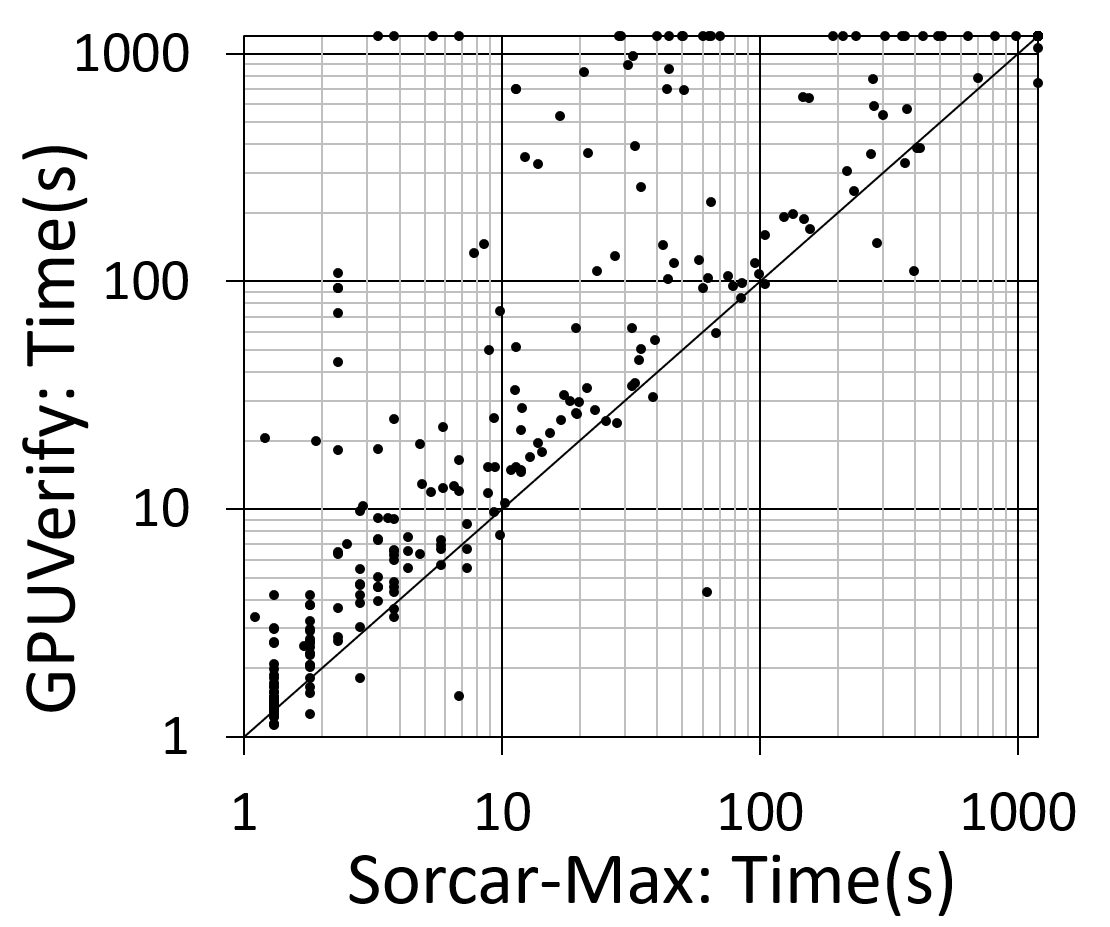
\includegraphics[width=6cm]{gpuTime.png} }}%
        \subfloat[]{{\label{sf:b}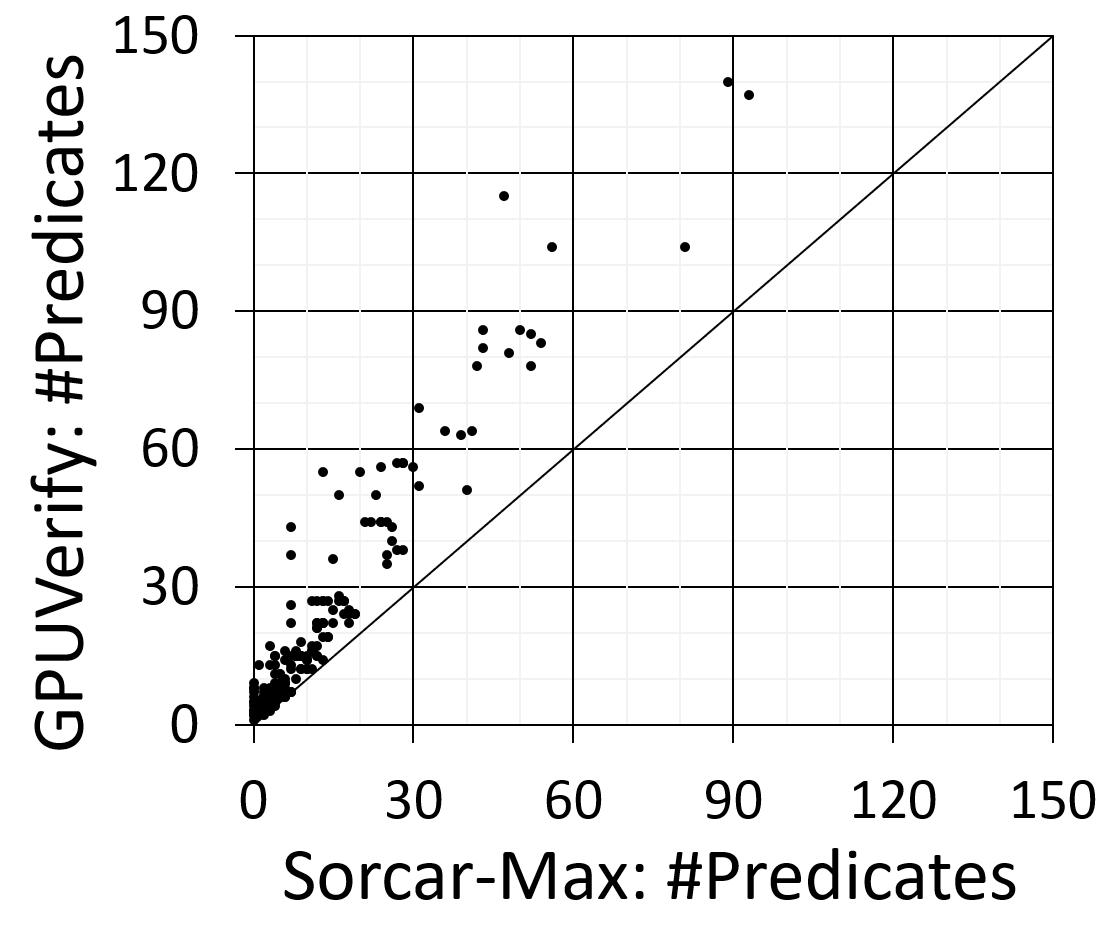
\includegraphics[width=6cm]{gpuPred.png} }}%
    }
    \\
    % 2. row
    \makebox[0pt]
    {    
        \subfloat[]{{\label{sf:c}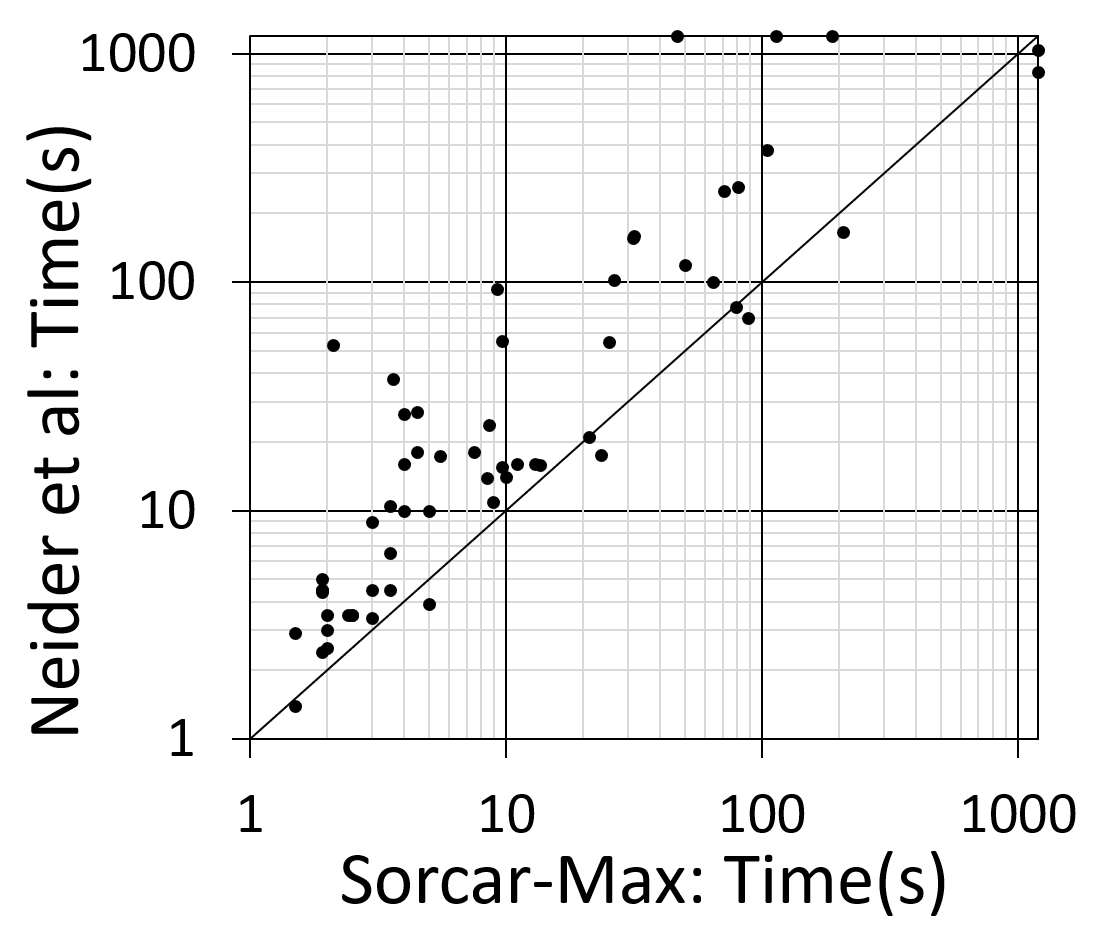
\includegraphics[width=6cm]{dryadTime.png} }}%
        \subfloat[]{{\label{sf:d}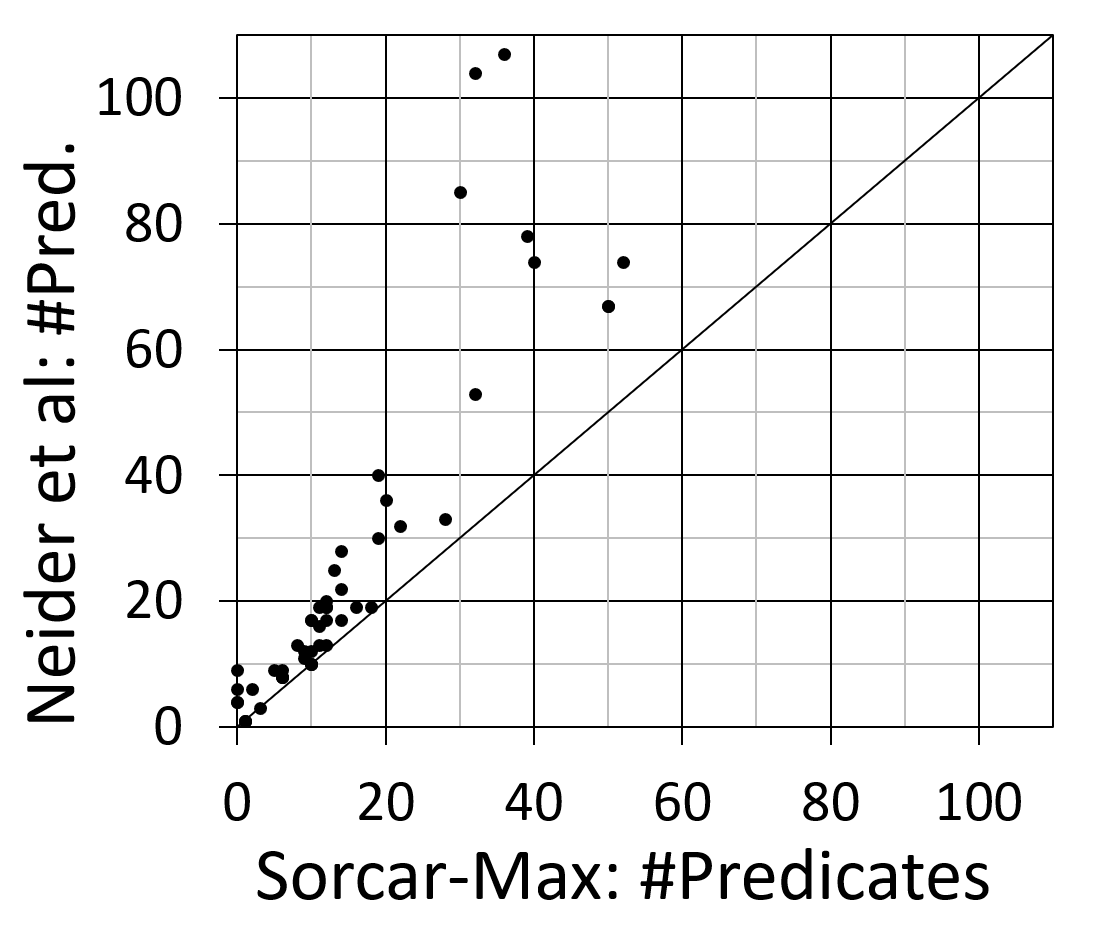
\includegraphics[width=6cm]{dryadPred.png} }}%
    }
    \\
    % 3. row
    \makebox[0pt]
    {
        \subfloat[]{{\label{sf:e}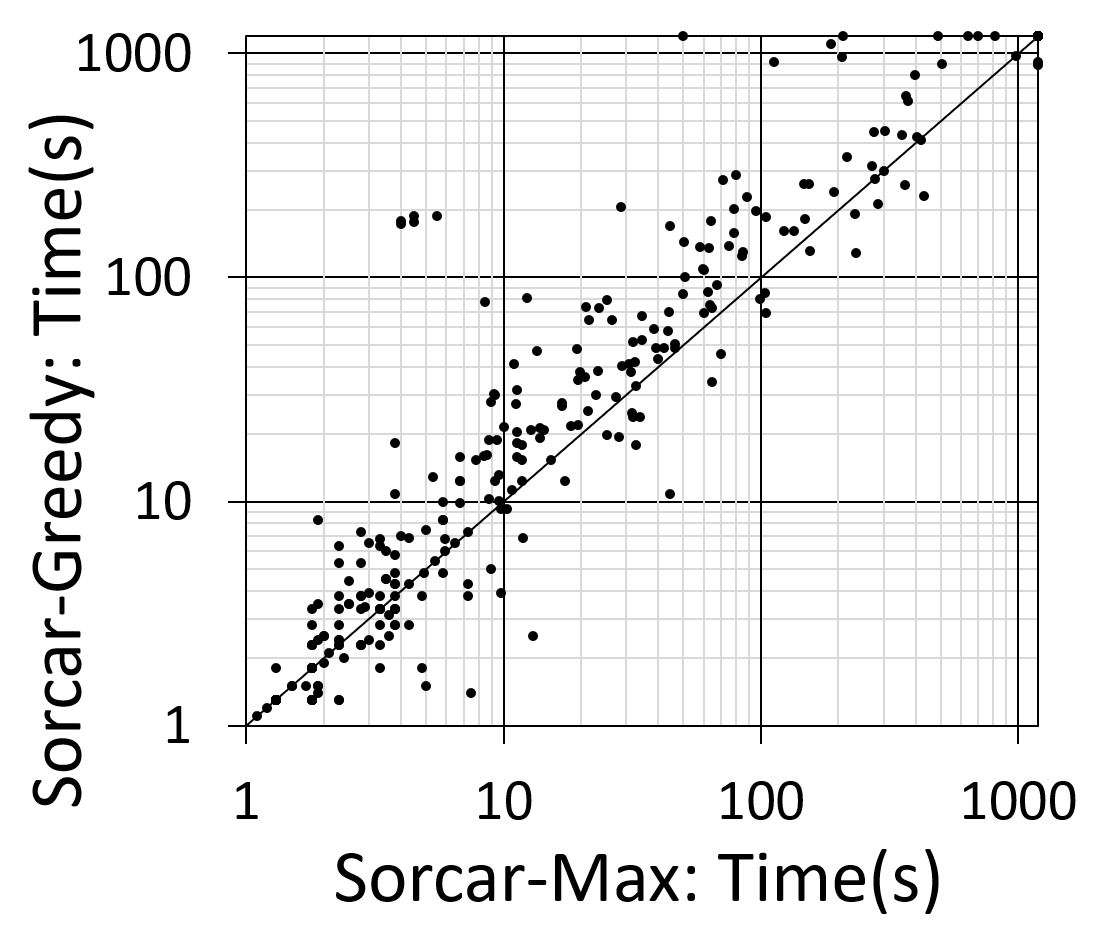
\includegraphics[width=6cm]{greedyTime.png} }}%
        \subfloat[]{{\label{sf:f}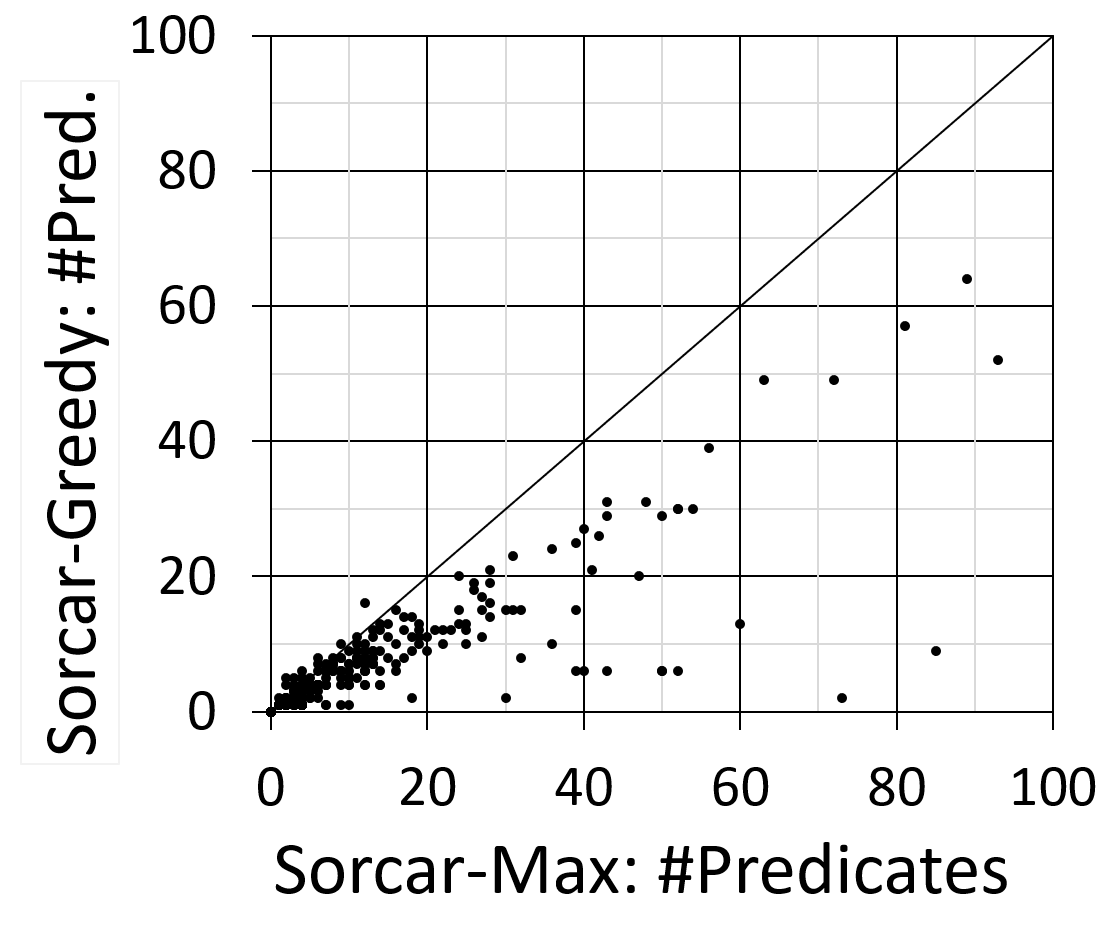
\includegraphics[width=6cm]{greedyPred.png} }}%
    }

    \caption{Comparison of time taken and number of predicates in final invariant, between the solvers \mbox{\sorcar-Max} and GPUVerify on Benchmark Suite\#1 ((a) and (b)), \mbox{\sorcar-Max} and Neider et al.'s tool on Benchmark Suite\#2 ((c) and (d)), and \mbox{\sorcar-Max} and \sorcar-Greedy over both benchmark suites (\ref{sf:e} and \ref{sf:f}).}
    \label{fig:results}
\end{figure}


%\paragraph{Implementation of Sorcar}
%\emph{Abstract Houdini} is a subframework in \boogie that allows extensions for loop invariant generation, and we implement the \sorcar algorithm (including all variants) using it.
%The algorithm is written in C+\!+ ($\sim 1800$ LOC).
%The benchmarks are transformed to the Abstract Houdini format for verification.


%---------- Evaluation ----------
\paragraph{Evaluation}
We have implemented all four variants of \sorcar in C+\!+ (approximately 1800 lines of code)\footnote{We will create an artifact and make the implementation publicly available.} and evaluated them on both benchmarks suits.
All experiments were conducted on an Intel Xeon E7-8857 v2 CPU at $3,6\,\text{GHz}$, running Debian GNU/Linux 9.5.
The timeout limit was $1200\,s$.
So as to not clutter the following presentation too much, we only report on the version of \sorcar that performed best: \textsc{Sorcar-Max} (using \RelevantPredicatesMax).
Additionally, we briefly compare \textsc{Sorcar-Max} to \textsc{Sorcar-Greedy}, which uses \RelevantPredicatesGreedy.\kern-.06em\footnote{All results can be found at \url{http://bit.ly/sorcar-evaluation}.}

Figures~\ref{sf:a} and \ref{sf:b} compare \textsc{Sorcar-Max} and GPUVerify on the first benchmark suite.
Figure~\ref{sf:a} compares the time taken by the two tools, while Figure~\ref{sf:b} compares the size of the final invariant (there is only one loop invariant in these programs).
%
As can be seen from the figures, \textsc{Sorcar-Max} compares significantly favorably in both time and size of predicates.
On programs that were able to verify, \textsc{Sorcar-Max} took on average $49\,s$ per program and synthesized invariants with an average number of $12$ conjuncts.
GPUVerify, on the other hand, took on average $96\,s$ per program and synthesized invariants with an average number of $23$ conjuncts.
Furthermore, \textsc{Sorcar-Max} was able to verify $22$ programs that GPUVerify could not verify, whereas GPUVerify verified only $2$ programs that \textsc{Sorcar-Max} could not verify. 

Figures~\ref{sf:c} and \ref{sf:d} compare \textsc{Sorcar-Max} to the tool of Neider et al.~\cite{DBLP:conf/tacas/Neider0MS018} on the second benchmark suite.
Again, \textsc{Sorcar-Max} outperformed the Houdini-based tool both in terms of time and size of invariants synthesized.
On programs that both were able to verify, \textsc{Sorcar-Max} took on average $24\,s$ per program and synthesized invariants with an average number of $25$ conjuncts.
On the other hand, Neider et al.'s tool took on average $75\,s$ per program and synthesized invariants with an average number of $41$ conjuncts.
Furthermore, \textsc{Sorcar-Max} was able to verify $3$ programs that the Neider et al.'s tool could not verify, whereas Neider et al.'s tool verified $2$ programs that \textsc{Sorcar-Max} could not verify. 

Finally, Figures~\ref{sf:e} and \ref{sf:f} compare \textsc{Sorcar-Max} and \textsc{Sorcar-Greedy}.
\textsc{Sorcar-Greedy} was slightly slower but was able to synthesizes, overall, much smaller invariants. 

%two versions of \sorcar, one that uses maximal set of relevant predicates (MAX) (Algorithm~2) and the one that uses the greedy method to find relevant predicates (GREEDY) (Algorithm~5). The greedy version of \sorcar performs a bit slower but is able to synthesizes, overall, much smaller invariants. 
%We also implemented the other variants  but we do not report on them here as the above two variants emerged as the most competitive.

%on the total time taken, and the size of the final invariant. Note that GPUVerify uses a prepossessing compilation step.  We subtract the time taken by this compilation step from the total time taken. 

%On the GPUVerify benchmarks, we evaluate the performance of the whole tool-chain, which includes a custom version of Boogie. We also set as baseline the performance of standard Boogie on the compiled Boogie programs. 
%For the Dryad benchmarks, we compare against the standard off-the-shelf Boogie.





%---------- Conclusion ----------
% 

\section{Conclusion}
\label{sec:conclusion}
Learning algorithms typically learn the simplest concepts that explain data.
\houdini is unusual in that it learns instead the \emph{largest} formulas that explain the data.
However, it has the nice property that it learns the invariant in a linear number of rounds.
In this paper, we have explored a new class of learning algorithms, \sorcar, that is parameterized by functions that add relevant predicates, and that are biased towards learning small invariants by being property-driven.
We have shown that these algorithms learn smaller invariants and prove programs correct significantly faster than state-of-the-art \houdini-based tools.

There are several future directions to pursue. First, we believe that further algorithms for learning conjunctions need to be explored. 
For instance, the Winnow algorithm~\cite{DBLP:journals/ml/Littlestone87} learns from positive and negative samples in time $\mathcal O(r \log n)$, where $r$ is the size of the final formula and $n$ is the number of predicates.
Finding Horn-ICE learning algorithms that have such sublinear round guarantees can be very interesting as $r$ is often much smaller than $n$ in verification examples.
Second, we would like to use the new \sorcar algorithms in specification mining settings where smaller invariants are valuable as they are read by humans.
Third, there are several type inference algorithms similar to \houdini (see~\cite{DBLP:conf/pldi/RondonKJ08}), and it would be interesting to explore how well \sorcar performs in such settings. 


%---------- Bibliography ----------
\bibliographystyle{splncs04}
\bibliography{bib}


%---------- Appendix ----------
\clearpage
\appendix
% !Tex root=main.tex

%---------- Variants of Sorcar ----------
\section{Variants of the Function \texttt{Relevant-Predicates}}
The following section presents the various variants of the function \texttt{Relevant-} \texttt{Predicates} in pseudo code.

%---------- Relevant-Predicates-Max ----------
\subsection{\texttt{Relevant-Predicates-Max}}
\label{app:relevant-predicates-max}

\begin{algorithm}[H]
        
    \Fn{\RelevantPredicatesMax{$N$, $H$, $X$, $R$}}
    {
    
        $R' \gets \emptyset$\;
    
        \ForEach{negative counterexample $c \in N$}
        {
            $R' \gets R'\cup \{ p \in X \setminus R \mid c \not\models p \}$\;
        }
    
        \ForEach{Horn counterexample $(\{ c_1, \ldots, c_n \}, c) \in H$}
        {
            $R' \gets R'\cup \bigcup_{i = 1}^n \{ p \in X \setminus R \mid c_i \not\models p \}$\;
        }
     
        \Return{$R'$}\;
    }
    
    \caption{Computing the maximal set of relevant predicates}
    \label{alg:relevant-predicates-max}
\end{algorithm}

%---------- Relevant-Predicates-First ----------
\subsection{\texttt{Relevant-Predicates-First}}
\label{app:relevant-predicates-first}

\begin{algorithm}[H]

    \Fn{\RelevantPredicatesFirst{$N$, $H$, $X$, $R$}}
    {
    
        Define a total order $<_\mathcal P$ over $\mathcal P$\;
        $R' \gets \emptyset$\;
    
        \ForEach{negative counterexample $c \in N$}
        {
            $R' \gets R'\cup \{ p \}$ where $p$ is the $<_\mathcal P$-smallest predicate with $p \in X \setminus R$ and $c \not\models p$\;
        }
    
        \ForEach{Horn counterexample $(\{ c_1, \ldots, c_n \}, c) \in H$}
        {
            $R' \gets R'\cup \{ p \}$ where $p$ is the $<_\mathcal P$-smallest predicate from the set $\bigcup_{i=1}^n \{ p \in X \setminus R \mid c_i \not\models p \}$\;
        }
     
        \Return{$R'$}\;
    }
    
    \caption{Computing relevant predicates based on a preference ordering}
    \label{alg:relevant-predicates-first}
\end{algorithm}

%---------- Relevant-Predicates-Min ----------
\subsection{\texttt{Relevant-Predicates-Min}}
\label{app:relevant-predicates-min}

\begin{algorithm}[H]

    \Fn{\RelevantPredicatesMin{$N$, $H$, $X$, $R$}}
    {

        For each $c \in N$, construct $A_c \coloneqq \{ p \in X \setminus R \mid c \not\models p \}$\;
        For each $(L, c) \in H$, construct $A_{(L, c)} \coloneqq \{ p \in X \setminus R \mid \exists c' \in L \colon c' \not\models p \}$\;    

        \BlankLine
        
        Compute a minimal hitting set $R'$ for the instance $Q \coloneqq \{ A_c \mid c \in N \} \cup \{ A_{(L, c)} \mid (L, c) \in H \}$ (e.g., using a SAT solver)\;
        
        \BlankLine

        \Return{$R'$}\;
    }
    
    \caption{Computing a minimal set of relevant predicates}
    \label{alg:relevant-predicates-min}
\end{algorithm}

%---------- Relevant-Predicates-Greedy -----------
\subsection{\texttt{Relevant-Predicates-Greedy}}
\label{app:relevant-predicates-greedy}

\begin{algorithm}[H]

    \Fn{\RelevantPredicatesGreedy{$N$, $H$, $X$, $R$}}
    {

        For each $c \in N$, construct $A_c \coloneqq \{ p \in X \setminus R \mid c \not\models p \}$\;
        For each $(L, c) \in H$, construct $A_{(L, c)} \coloneqq \{ p \in X \setminus R \mid \exists c' \in L \colon c' \not\models p \}$\;  

        \BlankLine
        
        $R'\gets \emptyset$\;
        $Q \gets \{ A_c \mid c \in N \} \cup \{ A_{(L, c)} \mid (L, c) \in H \}$\;

        \BlankLine

        \While{$Q \neq \emptyset$}
        {
            Pick $p \in X \setminus (R \cup R')$ such that $|\{ A \in Q \mid p \in A \}|$ is maximal\;
            $R'\gets R' \cup \{ p \}$\;
            $Q \gets Q \setminus \{ A \in Q \mid p \in A \}$\;
        }

        \BlankLine

        \Return{$R'$}\;
    }
    
    \caption{Greedily computing a ``small'' set of relevant predicates}
    \label{alg:relevant-predicates-greedy}
\end{algorithm}

\end{document}
